\documentclass{standalone}

\usepackage{times}
\usepackage{amsmath}
\usepackage{amssymb}

\usepackage[dvipsnames]{xcolor}
\usepackage{tikz}
\usepackage{tikz-qtree}
\usetikzlibrary{arrows,backgrounds,scopes}

\usepackage{pgfplots}
\pgfplotsset{compat=1.15}
\begin{document}
	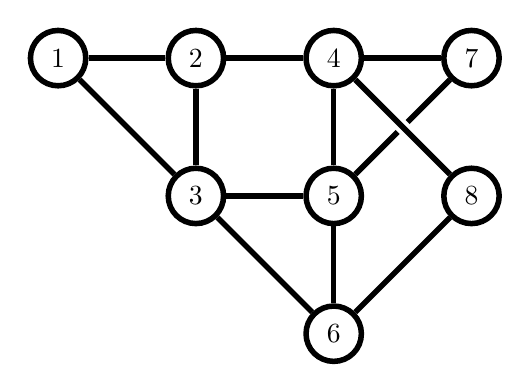
\begin{tikzpicture}[x=1.75cm,y=1.75cm,every node/.style={minimum width=2em,draw,circle,line width=2pt,},
		every edge/.style={draw, line width=2pt}]
		\node (v1) at (0,-0) {1};
		\node (v2) at (1,-0) {2};
		\node (v3) at (1,-1) {3};
		\node (v4) at (2,-0) {4};
		\node (v5) at (2,-1) {5};
		\node (v6) at (2,-2) {6};
		\node (v7) at (3,-0) {7};
		\node (v8) at (3,-1) {8};
		
		\draw (v1) edge (v2);
		\draw (v1) edge (v3);
		\draw (v2) edge (v3);
		\draw (v2) edge (v4);
		\draw (v3) edge (v5);
		\draw (v3) edge (v6);
		\draw (v4) edge (v5);
		\draw (v5) edge (v6);
		\draw (v4) edge (v7);
		\draw (v5) edge (v7);
		\draw (v4) edge[line width=5pt,white] (v8);
		\draw (v4) edge (v8);
		\draw (v6) edge (v8);
	\end{tikzpicture}
\end{document} 
